\documentclass[10pt, conference]{IEEEtran}

\usepackage{cite}
\usepackage{amsmath,amssymb,amsfonts}
\usepackage{algorithmic}
\usepackage{textcomp}
\usepackage{booktabs}
\usepackage{listings}
\usepackage{multirow}
\usepackage{graphicx}
\usepackage{subcaption}
\usepackage[hidelinks]{hyperref}
\usepackage{fancybox}
\usepackage{enumitem}
\usepackage{xcolor}
\usepackage[export]{adjustbox}
\usepackage{xspace}
\def\BibTeX{{\rm B\kern-.05em{\sc i\kern-.025em b}\kern-.08em
    T\kern-.1667em\lower.7ex\hbox{E}\kern-.125em X}}


\definecolor{listinggray}{gray}{0.9}
\definecolor{lbcolor}{rgb}{0.9,0.9,0.9}
\definecolor{dkgreen}{rgb}{0,0.5,0}
\definecolor{dkred}{rgb}{0.5,0,0}
\definecolor{gray}{rgb}{0.5,0.5,0.5}
\definecolor{cyan(process)}{rgb}{0.0, 0.72, 0.92}
\definecolor{safetyorange}{rgb}{1.0, 0.4, 0.0}
\definecolor{javagreen}{rgb}{0.25,0.5,0.35}
\definecolor{metalgrey}{rgb}{0.43, 0.5, 0.5}
 % comments
%basicstyle=\ttfamily\bfseries\footnotesize,


\lstdefinestyle{JavaStyle}{
    language=Java,      % choose the language of the code
    keywords=[2]{View, LayoutInflater, ViewGroup, Bundle, ListView, Fragment, Activity},
    keywords=[3]{onCreateView, inflate, getActivity, DLE, findViewById, setAdapter},
    keywords=[4]{@Override, listView, DirList},
    basicstyle=\ttfamily\bfseries,
    keywordstyle=\color[RGB]{69,97,189},
    keywordstyle=[2]{\color{cyan(process)}},
    keywordstyle=[3]\color{javagreen},
    keywordstyle=[4]\color{metalgrey},
    %safetyorange
    commentstyle=\itshape\color{green!60!black},
    moredelim=[l][\itshape\color{gray}]{//}, %<--- overrides line-comment style
    stringstyle=\color[RGB]{192,8,8},
    numberstyle=\itshape\color{yellow!50!black},
%   backgroundcolor=\color{lbcolor},
    tabsize=4,
%   rulecolor=,
    upquote=true,
    aboveskip={1.5\baselineskip},
    columns=fixed,
    showstringspaces=false,
    extendedchars=false,
    breaklines=true,
    prebreak = \raisebox{0ex}[0ex][0ex]{\ensuremath{\hookleftarrow}},
    frame=single,
    numbers=left,
    showtabs=false,
    showspaces=false,
    showstringspaces=false,
    %autodedent,%<--- removes indentation
}
\lstset{style=JavaStyle}

\newcommand\todo[1]{\textcolor{red}{#1}}
\newcommand\bears{\textsc{Bears}\xspace}

\begin{document}

\title{A Study of Multi-Location Bug Patches}

\author{Anonymous Authors}

%% JL: This is the author template from the IEEE example tex file.
%%
%% \author{\IEEEauthorblockN{1\textsuperscript{st} Given Name Surname}
%% \IEEEauthorblockA{\textit{dept. name of organization (of Aff.)} \\
%% \textit{name of organization (of Aff.)}\\
%% City, Country \\
%% email address or ORCID}
%% \and
%% \IEEEauthorblockN{2\textsuperscript{nd} Given Name Surname}
%% \IEEEauthorblockA{\textit{dept. name of organization (of Aff.)} \\
%% \textit{name of organization (of Aff.)}\\
%% City, Country \\
%% email address or ORCID}
%% \and
%% \IEEEauthorblockN{3\textsuperscript{rd} Given Name Surname}
%% \IEEEauthorblockA{\textit{dept. name of organization (of Aff.)} \\
%% \textit{name of organization (of Aff.)}\\
%% City, Country \\
%% email address or ORCID}
%% \and
%% \IEEEauthorblockN{4\textsuperscript{th} Given Name Surname}
%% \IEEEauthorblockA{\textit{dept. name of organization (of Aff.)} \\
%% \textit{name of organization (of Aff.)}\\
%% City, Country \\
%% email address or ORCID}
%% \and
%% \IEEEauthorblockN{5\textsuperscript{th} Given Name Surname}
%% \IEEEauthorblockA{\textit{dept. name of organization (of Aff.)} \\
%% \textit{name of organization (of Aff.)}\\
%% City, Country \\
%% email address or ORCID}
%% \and
%% \IEEEauthorblockN{6\textsuperscript{th} Given Name Surname}
%% \IEEEauthorblockA{\textit{dept. name of organization (of Aff.)} \\
%% \textit{name of organization (of Aff.)}\\
%% City, Country \\
%% email address or ORCID}
%% }

\maketitle

\begin{abstract}
    Automatic program repair is a promising approach for reducing the
    cost of quality assurance practices and faulty software. To date, most
    techniques proposed for test-driven automatic repair have succeeded
    primarily on bugs that benefit from short, single-location patches. Techniques
    that successfully generate multi-location patches often do so in an
    alternative, single-edit way, or by targeting particular multi-location bug
    patterns. Empirical studies of real-world similarly tend to focus on the
    patterns exhibited by single-location bug patches, and have not examined repairability
    of multi-location patches in detail. We present a comprehensive empirical analysis
    of multi-location patches for bugs in open source Java programs, focusing on static and
    dynamic properties that define the repair search space for a given bug.
    This analysis focuses on the key challenges of the dynamic program repair
    problem: the \emph{mutations and fix code} used to repair bugs in multiple locations;
    the \emph{fault locations} and their relationships; and the \emph{objective
      function}, and in particular how and to what degree test cases can be used
    (or not) to identify partial repairs. We identify key takeaways and
    challenges, with implications for future work in expressive, multi-location bug
    repair.
\end{abstract}

\begin{IEEEkeywords}
  software bugs, program repair
\end{IEEEkeywords}

\newcommand{\rqorinsight}[2]{
  \setlength{\fboxsep}{0.8em}
  \vspace{0.5em}
  \begin{center}
  \Ovalbox{\begin{minipage}{0.9\linewidth}
    \textbf{RQ#1:} #2
    \end{minipage}}
  \end{center}
  \vspace{0.5em}}

\section{Introduction}

%\renewcommand\todo[1]{}

\todo{TODO THROUGHOUT: virtually all of the figure/table captions are
  inadequate; they need takeaways.  Update those for which you're responsible,
  and make sure all tables/figures have a responsible person.}
Buggy software has a significant economic cost~\cite{cambridge-study}, and
software failures are estimated to have affected half of the world's
population~\cite{tricentis}.  This motivates research in
techniques to automatically find and fix bugs.  Some of these techniques have
begun to be integrated  which have become integrated into
real-world development practices~\cite{iceland,sapfix}.\footnote{https://engineering.fb.com/developer-tools/getafix-how-facebook-tools-learn-to-fix-bugs-automatically/}

A significant class of program repair techniques in both
\todo{update this citation list to include stuff published since 2017, plz}
research~\cite{genprog,angelix,Le17, Xuan17} and practice~\cite{sapfix} use test
cases to guide patch construction. At a high level, these techniques use test cases
to localize a defect --- identified by at least one failing test --- and to
validate which (if any) of the generated patch candidates lead
the program to pass all tests.
%
Patches are constructed in a variety of ways, ranging from heuristic, syntactic
\todo{as above, let's join the roaring 20s}
program manipulation~\cite{par,genprog,rsrepair,ae,prophet,hdrepair}, to specially adapted program
synthesis techniques~\cite{Konighofer11,Konighofer12,semfix,DeMarco14,angelix}. These techniques have successfully
repaired real, meaningful defects in large, complex
programs~\cite{angelix,genprog-eight-dollars,prophet,sapfix}.

Practically speaking, though, these techniques are typically limited in the types and
complexity of defects they can repair. Often this is by design: techniques may
limit the repair search space to single-location patches for
tractability~\cite{rsrepair,ae,hdrepair}, while others only target certain
classes of bugs~\cite{Xuan17,sapfix,DeMarco14,par}. However, even techniques
that can in principle generate repairs with multi-location patches typically
don't~\cite{patch-correctness}.
%
Meanwhile, many real-world bugs require multi-edit patches~\cite{d4j-dissection,zhong2015}, leaving a large
propertion of them  unrepairable by modern
research techniques in program repair.  
%Over half of the bugs in the popular bug
%benchmark Defects4J are patched by humans using multi-part
%patches~\cite{d4j-dissection}. Approximately 70\% of buggy source files in a
%large study of bugs in Apache projects required edits at two or more
%locations~\cite{zhong2015}.

This is a difficult problem.
A key tension in the design of an automated repair technique is the balance
between giving users confidence in patch correctness by maximizing its
subjective quality while managing a trivially-infinite search space. This space
is typically parameterized along several axes: (1) the \emph{fault space}:
potential program locations to be modified, (2) the \emph{mutation space}: which
modifications may be applied at a location, and (3) the \emph{fix space}: code
that may be instantiated for a specific mutation. For example, a repair
technique might identify the location of a null-pointer dereference (exploring
the fault space), decide to insert new code (mutation space), and synthesize
code to initialize the pointer (fix space). Many dynamic repair techniques can
be compared in terms of their choices along each of these axes, and traversal
strategies have first-order implications for scalability and for the type and
quality of patches produced.

Multi-location repair poses distinct challenges for each of these repair axes.
Spectrum-based fault localization~\cite{ochiai}, the most prevalent class of
fault localization used in program repair, does not specifically
identify sets of potentially-related locations; indeed,
the evaluation of most fault localization techniques typicaly assumes that a bug
is localized if any one buggy line is identified~\cite{fl-survey-wong}.
Some bugs \emph{are}
repaired in multiple locations using very similar
code~\cite{saha2019harnessing,jiang2019cmsuggester}, informing novel techniques
that constrain the \emph{fix space} of possible multi-location repairs accordingly.
But, one key question for applicability of these types of techniques is how prevalent
such bugs are, relative to bugs that require multiple
coordinating (but ultimately different) edits.
Note for example that over 50\% of the fixes in four 
Apache projects involve two or more entities -- i.e., a Java class, method, or field -- and 66\%-76\% of 
those multi-entity fixes involved syntactic dependencies~\cite{wang2018}. 
Test cases are used to evaluate candidate repairs in dynamic
repair techniques, but, anecdotally, may not be effective
at identifying partial repairs in a multi-location
context~\cite{better-fitness}.  
Although multi-location repair has been discussed in the context of other analyses
that study bug fix characteristics in general~\cite{d4j-dissection} as well as for
repair applicability specifically~\cite{zhong2015, wang2018}, to the best of our
knowledge there has been no significant previous study of the characteristics of
multi-location repairs in terms of their implications for automatic
repairability.  \todo{Something like: Instead, we chip away at pieces like the
  blind man at the elephant, or some some dumb analogy.  But punchy.}

To fill in this gap, and lay groundwork for more informed, systematic research
efforts in the space of multi-edit repair, we conduct a systematic study of real-world bugs with
multi-location patches.  We
look specifically at their characteristics with respect to the problem of the
automatic repair search space.  
We study bugs curated in two
real-world datasets that support program repair research: Defects4J~\cite{defects4j}
and \bears~\cite{bears}, in total, 1018 bugs in 51 projects.
% CLG asks: are these numbers accurate
More than half of these bugs were repaired by a
human developer using edits at multiple locations.  We look at characteristics along each of the
relevant axes of the program repair search problem: fault locations, mutation
operators, fix code, and evaluation (or fitness or objective) using test cases,
and find both important and, in some cases, unintuitive, implications for
automated techniques.  Our findings and contributions are:

\begin{itemize}
%\item An analysis and enumeration of multi-location patches in Defects4J and
%\bears.
% I think the above is addressed by the summary in the preceding paragraph.
\item \textbf{Fault Localization.}  We find that 58\% of multi-edit bugs have faulty locations that are not
  covered by all failing tests.  This is important because the assumptions underlying spectrum-based
  fault localization may not hold when used off-the-shelf for
  multi-edit bug repair, motivating the development of novel localization
  techniques. 
\item \textbf{Edit dependency.} We 
find that 45\% of bug patches contain dependent edits, and that such bugs
may be more difficult for current, state-of-the-art
techniques to automatically repair.  This means that APR techniques assuming edit
independence~\cite{hercules,theotherone} are applicable to a nontrivial propertion of complex bugs, while
still motivating development of new analyses that can reason about multiple,
related edits at once. 
\item \textbf{Cloning in multi-location repair} We find that over 30\% of bugs with multi-location
patches have very similar edits applied to different locations, suggesting the viability of 
program repair techniques designed to utilize code clones. Moreover, importantly, bugs in which 
none of the faulty locations are covered by all failing tests tend to include
such clones in their patches.  This suggests a path forward for predicting, a
priori, which type of technique may apply to a given bug. 
\item \textbf{Test cases for multi-edit patch validation.} We find that over 40\% of bugs with multi-location
  patches in Defects4J and over half in \bears do not require the edits at every
  location in their provided human patches to pass all test cases, suggesting
  that either patches contain unnecessary edits or that test cases
  do not fully capture the desired behavioral specification.  \todo{Think about
    how to ephrase this a bit more intuitively, and consider breaking up this
    bullet into multiple findings.} We also find that test 
  case based validation methods can positively identify close to 40\% of partial repairs,
  while less than
  20\% of partial repairs cause more test assertions to fail. Additionally, the 
  \emph{granularity} at which test suite behavior is measured (i.e., at the class,
  method, or assertion level) influences ability to identify partial
  repairs. 
\item dataset replication etc \todo{FIXME: Our dataset and analysis results,
    linked here anonymously, will be prettier for the camera ready we promise.}
\end{itemize}

In Section~\ref{sec:background}, we overview the problem domain to
motivate/outline our research questions, and characterize our datasets.
% We overview the key
%characteristics of the datasets that we use in our study in
%Section~\ref{sec:data-rq1}.  
We then describe the results of our study along the
three key axes of program repair: fault localization (Section~\ref{secFL}),
mutation operators and fix code (Section~\ref{sec:mutops}), and test cases as
the patch validation mechanism (Section~\ref{sec:tests}).  We conclude by
outlining limitations (Section~\ref{sec:limits}), related work
(Section~\ref{sec:related}).  Finally, 
% don't give up on this yet.  It's a complicated paper, roadmaps might actually
% meaningfully help
we summarize our takeaways for 
multi-location repair (Section~\ref{sec:takeaways}).

\section{Problem Definition}
\label{sec:background}

In this section we overview the background of automated program repair (APR) and
introduce key concepts that directly motivate our research questions.

\subsection{Automated Program Repair: a Search Problem}

The central goal of source-level automated program repair (APR) is to
automatically generate patches for bugs in programs. We restrict attention to
\emph{dynamic} or \emph{test-case guided} program repair, a prevalent class of
research techniques over the past decade~\cite{cacm19}.  Dynamic APR techniques
are characterized by their use of test cases that serve as the oracle for
program correctness, at least one of which is failing (i.e., exercises the bug
to be repaired).

At a high level, source level program repair is a \emph{search problem}, where
the objective is a set of source-level program edits that will cause it to pass
all of the provided tests. To do this, they first \emph{generate} a candidate
patch, then run the test suite to \emph{validate} it; for this reason they are
often called \emph{generate and validate} repair techniques. Generating a patch
requires navigating a search space, which is typically defined along the
following axes~\cite{ae,sqjo}:
\begin{enumerate}[wide]

\item \emph{Fault space.} The first problem with generating a patch concerns
  \emph{where} in the code a patch should be applied. Most dynamic repair
  techniques begin by using test cases as input to a fault localization
  technique. Such techniques identify (and typically score) suspicious code
  based on which test cases execute which pieces of code. Although the
  particulars of the fault localization employed can vary, most APR techniques
  use some variant of spectrum-based fault localization (SBFL)~\cite{ochiai} in
  this stage. The resulting computation defines the \emph{fault space}, or the
  candidate code locations considered for repair.

\item \emph{Mutation space.} After identifying a faulty program location, an APR
  technique must choose from the set of applicable modifications at the given
  point. Examples include GenProg's \emph{append}, \emph{replace}, and
  \emph{delete} mutation operators over statements~\cite{genprog-operators};
  PAR's human patch inspired edit templates~\cite{par}; and Nopol's condition
  replacement over \texttt{if} statements~\cite{Xuan17}. Although a larger
  mutation space allows the generation of a wider variety of patches with
  potentially more repairs, adding more mutations grows the entire generation
  search space combinatorially~\cite{long-search-spaces}.

\item \emph{Fix space.} Certain mutations must be instantiated with generated or
  selected code before they can be applied. For example, if a technique elects
  to insert a null pointer check, the specific object being checked for
  \texttt{null} must be chosen to generate a patch. This search space that must
  be navigated to instantiate a patch is referred to as the \emph{fix space}.
  The fix space can be quite large (or even infinite), and different APR
  techniques use different strategies to make it tractable. Some techniques
  tackle the problem by taking advantage of the \emph{plastic surgery
    hypothesis}~\cite{plastic}, which assumes that a bug can be repaired by code
  available in other parts of the same program. By contrast, learning-based
  approaches use models of code or repairs to inform
  modifications~\cite{prophet}, whereas synthesis-based approaches constrain a
  synthesis engine to a small vocabulary of fix ingredients, possibly informed
  by the code near the selected faulty location~\cite{angelix,s3}.
\end{enumerate}

After generation, patches must be validated. Candidate patches are typically
validated using the provided test cases as the objective function. In techniques
that require one, test cases can also be used as the \emph{fitness
  function}~\cite{genprog}; although some have supplemented the test case
objective with partial correctness measures like program
invariants~\cite{dinglyu}, memory snapshots~\cite{source-code-checkpoint}, or
similarity to human edits~\cite{hdrepair}, with maximization of tests passed
maintained as one of possibly many objectives.
%% JL: This might be too early, since we haven't talked about multi-location yet.
%% In a multi-edit context, ideally,
%% multiple tests would be able to idnetify partial repairs that could be composed.
%% However, evidence suggests that this does not always
%% apply~\cite{better-fitness,schulte}.

A practical implication of the size and complexity of this search space is
that APR techniques must engage in trade offs to render the problem tractable. 
Some techniques limit the \emph{fault space},
searching explicitly for single-edit patches~\cite{rsrepair,ae,hdrepair}.
\todo{let's add techniques post 2017 to this paragraph wherever they belong
  plz.}
All consider a constrained mutation space, varying in how constrained that space
is; some implicitly limit the mutation or fix space by targeting only certain
classes of bugs~\cite{Xuan17,sapfix,DeMarco14,par}. Regardless, even techniques
that can in principle generate repairs with multi-location patches typically
don't~\cite{patch-correctness}.
%
Meanwhile, many real-world bugs require multi-edit patches: over half of the
bugs in the popular bug benchmark Defects4J~\cite{defects4j} are patched by
humans using multi-part patches~\cite{d4j-dissection}. Approximately 70\% of
buggy source files in a large study of bugs in Apache projects required edits at
two or more locations~\cite{zhong2015}.

Our goal in this study is to understand what makes the generation of larger
patches difficult, and identify properties of these bugs and their associated
patches that can be exploited by future APR tools.  
We define this problem precisely and characterize our datasets next.

\subsection{Multi-Location Patches and Dataset}


We focus in this study on the properties of \emph{multi-location} patches. There are
several plausible definitions of multi- vs. single-location patches, with
implications for how they are studied. For the purpose of this study, we define
a \emph{patch location} as a contiguous sequence of edited lines of code.  We
combine two locations if one simply opens or closes a syntactic block inserted
by the other. That is, conceptually:
\begin{lstlisting}
+ Some_edit {
+ New code
  Existing code
+}
\end{lstlisting}
is treated as a single-location edit in our study. We ignore changes to
comments, whitespace, or \texttt{import} statements.
%
This intuitive definition is reasonably consistent with the general APR
paradigm. 
\todo{is it worth elaborating on which we exclude, anything that might be
  counterintuitive? Do we include declarations as separate edits? I know our
  philosophy is different from D4J, which is why I ask.}
%As a shorthand, we refer to bugs with multi-location human-written
%patches as \emph{multi-location bugs}.

\begin{table*}
\begin{center}
\begin{tabular}{l  rrr | rr | rr | rr}
\toprule
\multicolumn{10}{c}{\textbf{Defects4J}} \\
\midrule
Project & Bugs & Src (kloc) & Test (kloc) & \multicolumn{2}{c}{Multi-location} 
		& \multicolumn{2}{c}{Multi-test} & \multicolumn{2}{c}{Multi-location \&}\\
&&&&\multicolumn{2}{c}{bugs}&\multicolumn{2}{c}{bugs}&\multicolumn{2}{c}{Multi-test bugs}\\
\midrule
JFreeChart  & 26 & 193.3 & 74.6  & 11 & 42\% & 10 & 38\% & 7 & 27\%\\
Closure compiler & 174 & 150.6 & 112.6 & 55 & 41\% & 58 & 44\% & 31 & 23\%\\
Apache commons-lang & 64 & 57.8 & 47.4  & 32 & 49\% & 17 & 26\% & 13 & 20\%\\
Apache commons-math & 106 & 45.0 & 41.5 & 53 & 50\% & 28 & 26\% & 22 & 21\%\\
Mockito & 38 & 23.0 & 28.5 & 16 & 42\% & 18 & 47\% & 8 & 21\%\\
Joda-Time & 26 & 82.9 & 70.4 & 17 & 63\% & 13 & 48\% & 9 & 33\%\\
Apache commons-cli & 39 & 5.7 & 4.6 & 19 & 49\% & 13 & 33\% & 8 & 21\%\\
Apache commons-codec & 18 & 5.8 & 5.8 & 4 & 22\% & 9 & 50\% & 2 & 11\% \\
Apache commons-collections & 4 & 64.9 & 47.6 & 1 & 25\% & 0 & 0\% & 0 & 0\%\\
Apache commons-compress & 47 & 12.8 & 3.1 & 24 & 51\% & 9 & 19\% & 6 & 13\%\\ 
Apache commons-csv & 16 & 2.6 & 3.9 & 3 & 19\% & 3 & 19\% & 2 & 12\%\\
Gson & 18 & 16.8 & 12.8 & 6 & 33\% & 9 & 50\% & 5 & 28\%\\
FasterXML jackson-core & 26 & 27.9 & 8.1 & 13 & 50\% & 8 & 31\% & 5 & 19\%\\
FasterXML jackson-databind & 112 & 80.7 & 41.2 & 58 & 52\% & 14 & 12\% & 9 & 8\%\\
FasterXML jackson-dataformat-xml & 6 & 7.5 & 6.2 & 5 & 83\% & 2 & 33\% & 2 & 33\%\\
Jsoup & 93 & 7.9 & 2.2 & 32 & 34\% & 29 & 31\% & 21 & 23\%\\
Apache commons-jxpath & 22 & 28.7 & 7.6 & 16 & 73\% & 9 & 41\% & 8 & 36\%\\
\midrule
All (Defects4J) & 835 & 813.9 & 518.1 & 365 & 44\% & 249 & 30\% & 158 & 20\%\\
\midrule
\multicolumn{10}{c}{\textbf{\bears (single-module)}} \\
\midrule
FasterXML jackson-databind & 26 & 80.7 & 41.2 & 17 & 65\% & 4 & 15\% & 2 & 8\%\\
INRIA Spoon & 62 & 66.2 & 30.8  & 39 & 63\% & 23 & 37\% & 18 & 29\%\\
spring-data-commons & 15 & 45.8 & 28.8  & 9 & 60\% & 6 & 40\% & 2 & 13\%\\
traccar-traccar & 42 & 47.9 & 8.6 & 24 & 57\% & 3 & 7\% & 2 & 5\%\\
30 other projects & 38 & --- & --- & 22 & 58\% & 36 & 95\% & 9 & 24\%\\
\midrule
All (\bears) & 183 & $>$240.6 & $>$109.4 & 111 & 61\% & 72 & 39\% & 33 & 18\% \\
\midrule
Combined (Defects4J \& \bears) & 1018 & $>$1054.5 & $>$627.5 & 476 & 47\% & 321 & 32\% & 191 & 19\%\\
\bottomrule
\end{tabular}
\end{center}
\caption{\label{tab:dataset-characteristics} Characteristics of the Defects4J
  (top) and \bears (bottom) datasets.\todo{multi-location vs multi-test: don't
    belabor the point, but this caption should say SOMETHING about how to read
    the table.}}
\end{table*}

Our study requires a dataset of indicative, real-world,
multi-location defects.  We study both the defects in
Defects4J v2.0.0~\cite{defects4j} and \bears~\cite{bears}.  Table~\ref{tab:dataset-characteristics}
summarizes these datasets, both of which
consist of historical
bugs found in real world software projects. Defects4J contains 835 bugs from 
17 Java software projects, and is a popular dataset for evaluating 
program repair tools that target Java~\cite{durieux-repair-them-all}.\todo{add
  more references, there are other papers that use d4j to evaluate}
The dataset's patches are manually minimized to isolate the bug fix 
and exclude non-repair edits such as refactorings and feature additions.

With any dataset, however, there is a risk that tools may overfit
to the defects in question, and there is evidence that this situation applies to
program repair and Defects4J~\cite{durieux-repair-them-all}. 
We thus also study bugs from \bears~\cite{bears}, 
a set of Java bugs derived from failed Travis-CI builds of GitHub projects. 
\bears offers 251 bugs from 72 software projects, providing a greater diversity of 
projects compared to Defects4J. 
Several projects in \bears, however, are structured as multi-module projects, 
which are not currently compatible with our automation tools.
\todo{Is it worth expanding slightly on why/what this means?}
We thus limit our analysis of \bears to 183 bugs from 34 single-module projects.
\todo{what's going on with multi-location versus multi-test}

We start our analysis of multi-location patches by asking:
\rqorinsight{1}{How prevalent are human-written multi-location patches?}

Table~\ref{tab:dataset-characteristics} lists the numbers and percentages of
multi-location patches in Defects4J and \bears. 
We find that multi-location patches comprise 61\% of \bears and 44\% of Defects4J.
Although a multi-location human patch for a bug does not imply the 
non-existence of a simpler patch, the high proportion of bugs that have 
multi-location patches demonstrates the relevance of such bugs to fault localization and
program repair. 

\bears contains a greater proportion of 
multi-location patches compared to Defects4J. This may be the 
result of manual patch minimization in Defects4J
and lack thereof in \bears.
Thus, some \bears patches may be multi-location due to
non-corrective edits (e.g.: refactorings, feature additions).

Having established both that multi-location edits are common in real-world
programs, and established a suitable, plausibly indicative dataset to study
them, we decompose dynamic APR into multiple subproblems, driven by the
shape of the search problem it seeks to solve. We 
investigate properties of the multi-location fault space (Section~\ref{secFL}),
mutation and fix spaces (Section~\ref{sec:mutops}), and validation
(Section~\ref{sec:tests}). 

\section{Fault localization} \label{secFL}

%% what are the claims, what are we studying, why are we studying it

Spectrum-based fault localization (SBFL) is a commonly-studied dynamic
fault localization technique, and is often more effective than alternatives (like mutation-based fault 
localization~\cite{mut-analysis} or dynamic program
slicing~\cite{zou2019empirical}). It is a key first step to characterizing the
\emph{fault space} in automatic program repair; the majority of dynamic APR
techniques use some variant of SBFL for this purpose.

Fundamentally, the core assumption underlying SBFL is that \emph{failing tests
  execute buggy portions of the code relatively more often than passing tests.}
% Thus, if all failing tests execute a particular line of code, then that line of
% code is highly suspicious.  
SBFL techniques compute a suspiciousness by
measuring how often a line is executed by failing tests as compared to passing
tests, typically via some (linear) combination of their respective
coverage of a line.
% This suspiciousness score can be calculated a few different ways, but is
% typically a linear combination of the passing and failing test coverage. One of
% the oldest and commonly studied SBFL technique is Tarantula~\cite{tarantula}. In
% Tarantula, the suspiciousness score for a line $s$ is calculated by:

% $$\mathit{susp(s)} 
% =\frac{\mathit{\%F(s)}}{\mathit{\%F(s)} + \mathit{\%P(s)}}$$

% where  $\mathit{\%F(s)}$ and $\mathit{\%P(s)}$ are, respectively, the percentage of failing 
% tests and passing tests that execute $s$. There are newer, more effective 
% SBFL techniques that calculate this score differently, such as Ochiai~\cite{ochiai} and 
%DStar~\cite{wong2013dstar}. 
SBFL techniques include but are not limited to Tarantula~\cite{tarantula},
Ochiai~\cite{ochiai} and DStar~\cite{wong2013dstar}; in general, though more
recent approaches are typically more effective, such approaches tend to localize similar
faults~\cite{zou2019empirical}.

Assigning a suspiciousness score to each line of code is well-suited to single
location repair. Indeed, the evaluation of most SBFL techniques asks exactly the
question of interest when considering a technique's suitability for
single-location repair: how often does a given technique assign high scores to 
individual buggy lines of code?

Such evaluations, by and large, do not consider the implications of
suspiciousness scoring in a multi-location repair context.  Instead, evaluations
typically consider a technique ``successful'' if it identifies \emph{any} of a
set of changed lines as highly-ranked or likely-suspicious.  While appropriate
for the question being asked in such evaluations, this does not address
suitability for multi-location program repair.%  Identifying one of several buggy
%locations is generally inadequate in a context where multiple locations must be
%modified. 
We investigate how well the SBFL assumption
applies to tests that identify bugs that require multi-location patches, asking: 

\rqorinsight{2}{Do failing tests of a multi-location bug execute all the same patch locations or 
all different patch locations?}

We focus especially on bugs that are associated with multiple failing tests: a bug
with only a single failing test trivially and equally implicates all the lines
that test executes.  If multiple tests cover the modified locations well, then
SBFL's core assumption holds and multi-location repair can expect to effectively
make use of the off-the-shelf ranking these techniques currently provide
(indeed, this has been tried~\cite{angelix}). If not---that is, if multiple
tests exercise \emph{different} portions of the buggy code---SBFL off-the-shelf
will by definition be less effective in guiding APR to correctly modifying
multiple buggy locations at once.
Fundamentally, we ask whether multiple failing tests cover exactly the same
patch locations, exactly disjoint patch locations, or some combination.

\todo{I think this RQ doesn't have enough context for the reader to understand
  what it's about at this point.  Please add some text to give more
  explanation/motivation for it.}
In addition, for purposes of fault localization, we want to know if we can detect 
whether tests will cover disjoint or same fault locations given only the buggy code. 
Thus, we also ask:

\rqorinsight{3}{Do tests that cover different (resp. same) fault locations also cover different 
(resp. same) code locations in general?}

\todo{Throughout methodology and results: rename disjoint/overlap/identical on
  both charts and in text, update text accordingly.  Include caveat to mitigate
  identified risk of new naming.}

\subsection{Methodology}

Between both datasets, there are 191 total bugs that both require multi-location
patches and contain multiple failing tests. However, we were not able to obtain coverage 
data for one of the bugs in Bears, leaving 190 total bugs: 158 in Defects4J, and 32 in
Bears. 
For each of these bugs, we used JaCoCo\footnote{https://www.eclemma.org/jacoco/}
to determine which code locations in both the buggy and patched versions were executed
(at least once) by each failing test.

To answer RQ2, we used the patch locations that were executed by the tests to categorize 
each bug into three \emph{coverage patterns}, as follows:
\begin{itemize}
\item \emph{disjoint} bugs are those for which no line in the patch is covered by all
failing tests.  Intuitively, these are the bugs for which the core SBFL
assumption is violated.
\item \emph{overlap} bugs are those for which some patch lines are covered
by all failing tests, but some are only covered by a subset of the failing
tests. These bugs also violate the core assumption of SBFL, albeit to a lesser
extent.
\item \emph{identical} bugs are those for which all tests cover the exact same
  set of patch lines.
\end{itemize}

In our experiments, we classify bugs using coverage of the patch lines, as opposed to 
coverage of 
patch locations (where a patch location is considered covered if any line at that patch location 
is 
executed). For the purposes of fault localization, coverage of patch locations is more valuable 
than coverage of patch lines, and we analyzed 66 Defects4J bugs\footnote{All 
bugs in Defects4J version 1, because of the way we calculate coverage information.}
 and all the Bears bugs, a total of 98 bugs, to see whether categorization 
based on patch line 
coverage matched categorization based on patch location coverage.

To answer RQ3, we took all code locations executed by tests in the buggy version and
calculated the percentage of lines that were executed by all failing tests. 
A lower percentage indicates that the failing tests execute different portions of the buggy 
code, whereas a higher percentage indicates that the failing tests all execute a similar
set of code, corresponding to bugs we expect to be \emph{disjoint} and \emph{identical},
respectively.

After calculating the percentages, we split the bugs based on whether we categorized the bug 
as \emph{disjoint}, \emph{identical}, or \emph{overlap} in the previous experiment.
We qualitatively observed the degree to which the percentage corresponded to its coverage 
pattern. \todo{Use a real statistical measure}\todo{Yes, really.}

\todo{Combine these three figures into 1}

\begin{figure}
	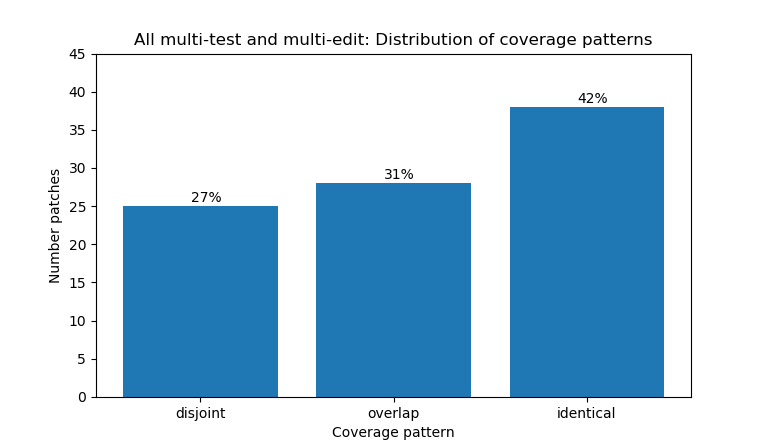
\includegraphics[width=\linewidth]{img/coverage-all.png}
	\caption{Distribution of coverage patterns for bugs with multiple failing
      tests that are repaired with multi-location patches in Bears and Defects4J.}
	\label{fig:coverage-all}
\end{figure}


\begin{figure}
	\begin{subfigure}{\linewidth}
		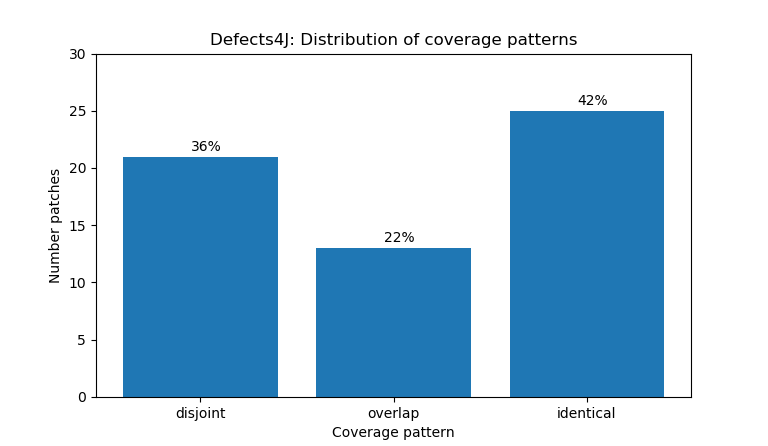
\includegraphics[width=\linewidth]{img/coverage-d4j.png}
		\caption{Distribution of coverage patterns for Defects4J.}
	\end{subfigure}

\vspace{0.5cm}

	\begin{subfigure}{\linewidth}
		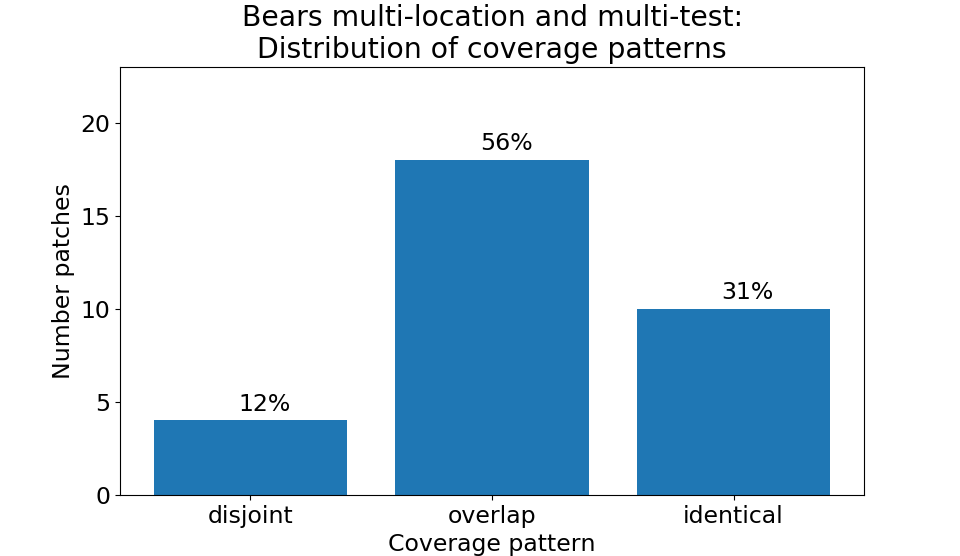
\includegraphics[width=\linewidth]{img/coverage-bears.png}
		\caption{Distribution of coverage patterns for Bears.}
	\end{subfigure}
	\caption{Distribution of coverage patterns by dataset,
          indicating significant differences between the multi-location bugs in
          Bears and Defects4J.}
	\label{fig:coverage-datasets}
\end{figure}

\subsection{Results}

\subsubsection{Distribution of Coverage Patterns} \label{sec:cov_patterns}

Figure~\ref{fig:coverage-all} shows results for the overall distribution of coverage patterns, 
answering RQ2. 
For a 29\% bugs, none of the patch lines were executed by all failing tests as they were 
shown to be \emph{disjoint}.  An almost equal proportion of bugs, 32\%, were classified as 
\emph{identical}, indicating that all failing tests executed the same patch lines.
In addition, another 39\% were classified as \emph{overlap}, exhibiting a combination of the 
\emph{disjoint} and \emph{identical} characteristics.

Note, however, that the behavior varies considerably by dataset;
Figure~\ref{fig:coverage-datasets} shows results. In Defects4J, the patterns all have similar 
numbers of bugs, while in Bears, there are fewer \emph{disjoint} bugs and more 
\emph{overlap} 
bugs.
We hypothesize that this may be due to differences in how the two  
datasets were selected and constructed:
The Defects4J dataset specifically enforces a requirement that the patches in the 
dataset be isolated, i.e., not containing any refactorings or new features, to improve the 
usability of the dataset. The authors specifically chose patches that met this requirement, 
and in some cases, manually isolated the bug themselves~\cite{defects4j}. By contrast, the 
bugs in 
Bears are scraped directly from continuous integration systems, and the 
only requirements for inclusion is that the bug must be reproducible and that
the patch must be written by a human. In addition, Bears was designed to be evolvable 
and relatively easily expanded as a dataset, which is at odds with manual inspection and isolation of 
bugs~\cite{bears}.
Given that these two datasets were designed with different values and demonstrate very 
different behavior, these findings highlight the importance of using diverse datasets in 
evaluating program repair techniques.

Out of the 98 bugs we checked, only seven bugs had differing coverage patterns when 
classified based on coverage of patch lines vs. coverage of patch locations. All seven of these 
bugs 
were classified as \emph{overlap} when classified by line coverage, but were classified as 
\emph{identical} when classifying by patch coverage, indicating that all the failing tests were 
executing different paths within the same patch locations. \todo{Is this discussion confusingly 
worded? Because patch locations refer to the patch chunk, made up of one or more lines of 
code.}

Overall, SBFL assumes that faulty locations are executed more often by identifying 
or failing test cases and is not designed to find many of these multi-location
faults. Our results suggest that off-the-shelf SBFL techniques are not
well-suited to guiding APR techniques that conform to the dominant paradigm to repairing
these types of multi-location, multi-test bugs.

\begin{figure}
	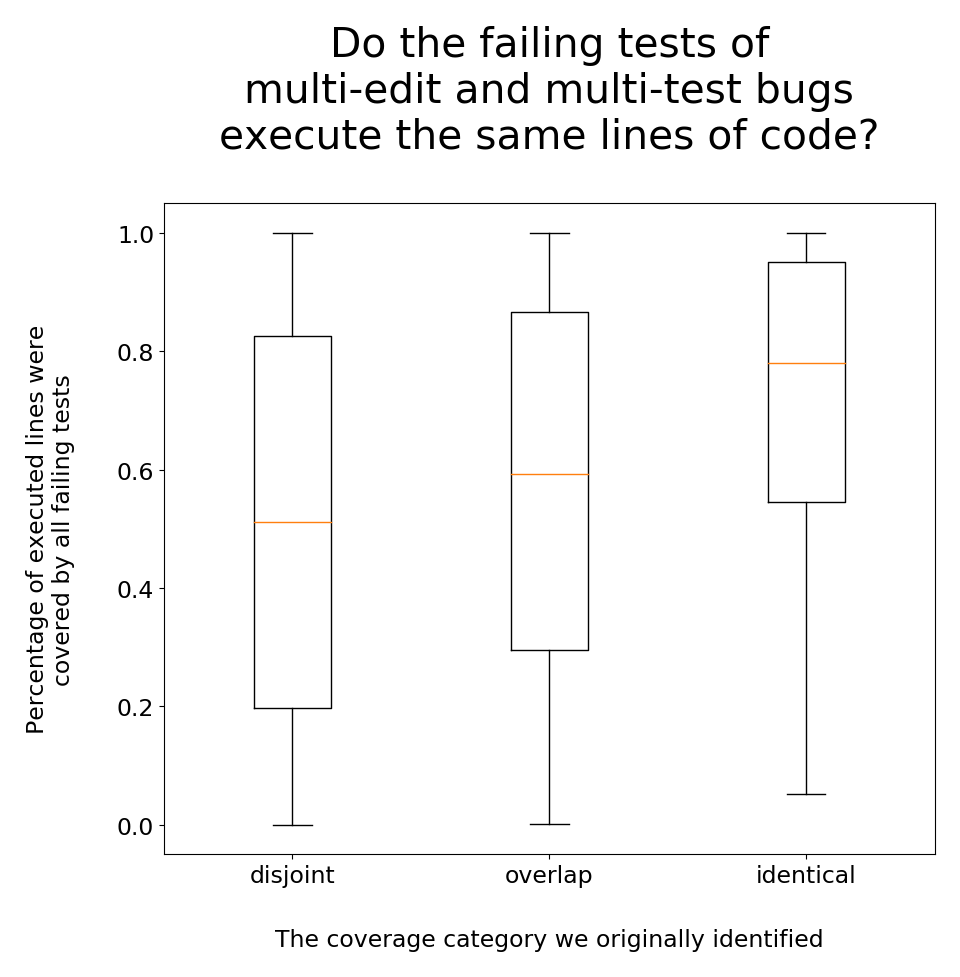
\includegraphics[width=.9\linewidth,left]{img/coverage-buggy.png}
	\caption{Boxplots representing the distribution of bugs based on it's percentage of lines 
	executed 
	by all failing tests. A bug scored at 100\% indicates that all failing tests executed the same 
	lines of 
	code, whereas a bug scored at 0\% indicates failing tests all executed different lines of 
	code. 
	These boxplots are split by coverage pattern, as categorized before.}
	\label{fig:coverage-buggy}
\end{figure}

\subsubsection{Generalization of Coverage Patterns}
\todo{As above, this question doesn't have enough motivation/context, so as a
  reader I'm struggling to figure out what we're asking/why the answer matters.
  This problem may be solved by fixing the text above, but it may require some
  text here as well.}
Our results in Figure \ref{fig:coverage-buggy} answer RQ3. Here, we see three distributions, 
separated by coverage pattern, and plotted based on the percentage of lines executed by all 
failing tests. 

The distributions of \emph{disjoint} bugs (and to a lesser extent, \emph{overlap} bugs) are 
distributed almost uniformly across the 0\% to 100\%, indicating that \emph{disjoint} bugs are 
not more or less likely to have failing tests that cover the same or different parts of the code 
base. Note that a bug categorized as \emph{disjoint} can be scored 100\%, as the 
patch can introduce if statements that change the control flow.

In contrast, we can qualitatively observe that \emph{identical} bugs are more likely to have 
failing tests that execute the same lines of code, as we might expect. However, this is not a 
definitive characteristic, as \emph{identical} bugs in our dataset scored anywhere between 
5\% to 100\%.

From these observations, we conclude that the degree to which failing tests cover the buggy 
code are not effective predictors for the eventual coverage pattern for the bug. 


\section{Mutation Operators and Fix Code}
\label{sec:mutops}

Given suitably selected fault locations, APR techniques vary in the types of
mutation operators they consider, how they select between them, and how they
select new fix code to instantiate them, as necessary. 
%  For example, a na{\"i}ve
% approach with only \texttt{insert}, \texttt{replace}, and \texttt{delete}
% operators must choose between them at a location and, in the case of
% \texttt{insert} and \texttt{replace}, choose code to insert/replace at that
% location.  
%
The few techniques that handle or at least enable multi-edit patches vary in their
handling of mutation operator selection and instantiation.  At one
extreme, semantics-based repair~\cite{s3,angelix} can represent dependent edits between multiple
locations as a conjunction of multiple constraints to simultaneously solve,
bounded by some number of edits and code components that are computationally feasible. 
At the other extreme, search-based or
evolutionary techniques~\cite{genprog,par} typically treat different mutation
operators independently, relying on the search to 
% That is, a modification in one location does not
%inform the selection of a modifications to apply in a second location; instead,
%the heuristic search is trusted to 
identify copacetic combinations.  The size of
the search space increases combinatorially in this context, however, rendering
the chances of finding suitable multi-edit repairs without additional guidance
quite low~\cite{ae,long-search-spaces}. Accordingly, heuristic multi-location
techniques~\cite{saha2019harnessing} make assumptions about the 
shape of the search space, 
targeting in particular bugs that can be repaired by multiple syntactically similar pieces of
fix code.

Note that the types of edits included in human patches has been
studied~\cite{examples}, with references for both search space size generally
and, potentially, patch quality~\cite{moreexamples}.  Here, we are especially
concerned about the 
\emph{relationships} between multiple edits, because such relationships have
key implications for how edits should be designed, selected, and instantiated 
in automatic multi-location repair. 

\subsection{Dependencies}

One of the dimensions of the relationship between multi-location patches is potential
\emph{dependency} between the edits, because edit dependency can and should
inform how those edits are selected and applied (i.e., consider the difference
between a multi-location
bugs repaired by applying the same independent edit in four places, as
compared to a bug repaired by applying  four control- and data-dependent
modifications).  Specifically, we ask:
\todo{This is our second RQ3}
\rqorinsight{3}{How prevalent are dependencies between edited code in
  multi-location patches?}

To answer this question, we broaden the scope of multi-location patches to 
include all patches containing at least two added, removed, or modified lines, 
again ignoring edits to comments, whitespace, or imports.
\todo{why?  And, which part of Table 1 shows this set?  Or should we be modifying the
text in the previous section?}
This expanded dataset contains 659 Defects4J v2 and 151 \bears bugs.
We consider a patch to contain \emph{dependent edits} if there exists 
control or data dependencies between added, deleted, or modified statements.
We analyze deleted/modified statements in the pre-patch code 
and added/modified statements in the post-patch code for
dependencies.\todo{Somehow, I'm not able to parse this preceding sentence.}
  
For practical performance and scalability reasons, 
we perform intraprocedural analysis. 
We do, however, gather some interprocedural data dependency information 
using the following heuristics:
\begin{itemize}
	\item We treat all method call statements as dependent on all variables
          passed as arguments. 
	\item If a statement invokes a getter method \texttt{Class.getX()} 
          we heuristically  assume that the statement reads \texttt{Class.X},
          whether or not \texttt{Class.X} exists.
	\item If a statement invokes a setter method \texttt{Class.setX()}, 
	we again heuristically assume that the statement writes to \texttt{Class.X}. 
\end{itemize}

\todo{We need one more paragraph acknowledging the limitations, here, or a
  little more detail above. Is this is a sound overapproximation?  Do we reason
  about aliases at all?  We wrote this code? Is it in our replication package?}

\paragraph{Results}

We find that 40\% of Defects4J patches, 63\% of \bears patches, 
and 45\% of the combined datasets' patches contain dependencies 
between edited statements.
Our finding supports earlier results on edit dependencies in 
bug patches~\cite{zhong2015}.\todo{Preceding sentence, and honestly likely this
  whole paragraph, is redundant with the last paragraph of this results
  subsection.  I think this redundancy can be reduced by fixing the RQ to
  actually match the question being asked in this subsection.}
Patches with and without edit dependencies both form a substantial
portion of multi-line patches,
and neither type of patch should be ignored.\todo{Are these results in a table
  somewhere? Short answer is ``only kind of, but it's hard to reference right
  here because the table answers a sort of different question.'' See below for
  my suggestion on changing the question.}

\begin{table}
{\begin{center}
	\begin{tabular}{l  rr  rr  rr}
		\toprule
		\multicolumn{7}{c}{\textbf{Patches with Dependent Edits}} \\
		\midrule
		APR (RepairThemAll) & \multicolumn{2}{c}{Defects4J} & \multicolumn{2}{c}{\bears} & \multicolumn{2}{c}{Combined} \\
		\midrule
		Success by any tool & 43 & 32\% & 9 & 9\% & 52 & 23\% \\
		Failure by all tools & 93 & 68\% & 86 & 91\% & 179 & 77\% \\
		Not evaluated & 130 & --- & 0 & --- & 130 & --- \\
		\midrule
		Total evaluated & 136 & 100\% & 95 & 100\% & 231 & 100\% \\
		Total & 266 & --- & 95 & --- & 361 & --- \\
		\midrule
		\multicolumn{7}{c}{\textbf{Patches without Dependent Edits}} \\
		\midrule
		Success by any tool & 96 & 57\% & 7 & 13\% & 103 & 46\% \\
		Failure by all tools & 73 & 43\% & 49 & 87\% & 122 & 54\% \\
		Not evaluated & 224 & --- & 0 & --- & 224 & --- \\
		\midrule
		Total evaluated & 169 & 100\% & 56 & 100\% & 225 & 100\% \\
		Total & 393 & --- & 56 & --- & 449 & --- \\
		\bottomrule
	\end{tabular}
 \end{center}
}
	\caption{Multi-line patches with respect to the presence of 
	dependent edits and whether any APR tool successfully 
	repaired the bug in RepairThemAll~\cite{durieux-repair-them-all}.
	Bugs categorized as {\normalfont Not evaluated} are those introduced in 
	v2 of Defects4J, which RepairThemAll didn't study.\todo{Is it possible
          or reasonable for this to be one or more Venn diagrams instead?}}
	\label{tab:dependency-repair-contingency-table}
\end{table}

\todo{Feels like these results come out of nowhere/are not associated with an
  RQ.  Can we modify the RQ to include this question in its scope? That would be
  nice and add clear novelty to answering it.  The text here should be updated
  to reflect that it's answering an RQ in that case.}
We further compare how often APR techniques 
successfully repair bugs whose patches do (not) contain edit dependencies.
Table~\ref{tab:dependency-repair-contingency-table}
show the frequencies and percentages of multi-line patches with respect to edit dependency 
and whether an APR tool successfully repaired bug in 
RepairThemAll~\cite{durieux-repair-them-all}, a repair experiment running 
11 APR tools on 5 benchmarks, including Defects4J v1 (containing a subset of Defects4J v2) and \bears.

We find that the presence of edit dependencies 
reduces the likelihood of APR tool success for Defects4J bugs.
Using a $\chi^2$ test, we find a statistically significant relationship ($p < 0.001$)
between APR success and the presence of edit dependencies for Defects4J patches. 
We fail to find statistically 
significant relationships over \bears patches, likely due to the small number (16) of 
successfully auto-repaired \bears bugs with multi-line human patches.
The generally lower auto-repairability of bugs with edit dependent patches compared 
to their non-edit dependent brethren suggest that such dependencies indeed 
add complexity to the search for a repair.\todo{What happens if we aggregate the
  two datasets? Do we have a good (scientific) reason to treat them separately?
  (I'm kind of thinking, what's the point of using both datasets if we don't
  aggregate them to get more statistical power....)}

Our results substantiate prior research~\cite{zhong2015} on the frequency of 
bugs with dependent edits in human patches. A diverse range of APR 
techniques are less likely to repair such bugs. Dependent edits, however, may 
be an opportunity to constrain the search space by creating constraints between 
otherwise independent mutations. There is an opportunity to profit from edit 
dependencies to repair a large class of difficult bugs.


\subsection{Cloned code}

In addition to dependency, multi-location patches can be related through syntactic
similarity. That is, a patch can consist of a code edit applied repeatedly in
multiple locations. Thus, we ask the following research question:

\rqorinsight{4}{How often do code clones occur in multi-location bugs? Is the existence of 
	code
	clones in human patches correlated with specific patterns of fault localization?}

Previous work~\cite{wang2018} suggests that one potential fruitful way to enhance
APR techniques is to allow them to apply a single edit to multiple locations.
This is based on the observation that human developers tend to make exactly the 
same edits in multiple locations when fixing bugs. 

As a proxy for measuring how often this style of repair actually occurs, we seek
to understand the 
prevalence of code clones in human patches. If a large proportion of multi-location bugs contains code 
clones, then we can corroborate the usefulness of previous repair techniques that specifically apply 
similar 
edits for a bug~\cite{saha2019harnessing}.

We further attempt to correlate the coverage patterns outlines in
Section~\ref{secFL} with the existence of code clones in human patches.  Our 
intuition is that a \emph{disjoint} bug may be more likely to occur when a
developer needs to apply the same fix at multiple independent locations, that
can or should be tested separately.  We therefore 
 hypothesize that \emph{disjoint} bugs will have a higher incidence of code
clones. By contrast, bugs categorized as \emph{same} or \emph{overlap} may have
more inter-related parts that are not merely the same statements copied to
multiple locations.

%Possible intuition: if we can find some kind of correlation between fault localization results
%and code clones, then if some APR research decided to follow Wang et al's suggestion and
%include "repeat same edits at multiple location" operator, then our results may advise
%the APR to be more likely to apply the repeat edit operator when the fault localization
%result matches specific patterns.

\subsubsection{Methodology}
\label{sec52}
Our dataset includes all multi-location bugs excluding those with more than 6 faulty locations to 
constrain the search space, leaving 216 bugs to analyze. We determine the existence of code 
clones through manual inspection.

% We cross validate our list of bugs with clones with results from previous work proposing and 
%evaluating an APR tool named Hercules~\cite{saha2019harnessing}. Hercules is a generate and 
%validate approach that could also exploit similar code locations to generate patches with code 
%clones. It was evaluated with the bugs in Defects4J version 1, which consists of 395 total bugs 
%and 187 multi-location bugs. 

In comparing these results with the results of the coverage experiment in
Section~\ref{secFL}, we focus on the multi-test and multi-location bugs used in the coverage 
experiment and exclude bugs with more than 6 faulty locations, leaving 166 bugs.

We call the edits at two locations code clones if it is one of the following four cases:
\begin{enumerate}
	\item Same Case: The two locations are alpha-equivalent. 
	\item Literal Case: The two locations differ by at most one constant or arithmetic operator,
	or replacement of one constant with variable.
	\item Composite Case: The patch at one location is exactly copied and contained within the patch at 
	the 
	second location (the second location  has additional lines in the patch).
	\item Move Case: Two locations forms a "movement" of code (i.e., one location is an insertion of 
	code 
	while the other is a deletion of the same code, essentially moving the code from one location to 
	another).
\end{enumerate}

\subsubsection{Results}

\begin{table}
{\begin{center}
\begin{tabular} {lrrr}
\toprule
& Defects4J & \bears & Combined \\
\midrule
Same & 71 & 9 & 80  \\ 
Literal & 23 & 2 & 25  \\
Composite & 11 & 1 & 12  \\
Move & 11 & 1 & 12  \\
\midrule
Any & 108 & 13 & 121  \\
No clones & 200  &  51 & 251 \\
Total & 308 & 64 & 372 \\
\% with Clones & 35.1\% & 20.3\% & 32.5\% \\
\bottomrule
\end{tabular}
\end{center}
}
\caption{Code clone information for multi-location bugs. 
     \emph{Same}, \emph{Literal}, \emph{Composite} and \emph{Move} correspond to the
    four types of code clones considered, as described in Section~\ref{sec52}. ``Any'' means the bug
    contains any of the four types of clone; some bugs contain
    pairs of clones that belong to different categories. 
    Over
    30\% of multi-location bugs has code clones.}
\label{tab:clones}
\end{table}

As shown in Table~\ref{tab:clones}, out of the 372 multi-location bugs,
121 of them, or  32.5\%, included at least one type of cloning between fault locations, indicating a 
significant 
prevalence of code clones in multi-location human patches.
Note that "Any" may not
be the sum of the previous four rows because some bug could contain multiple pairs of code clones 
that
belong to different categories.


\begin{table}
{\begin{center}
\begin{tabular} {lrrrr}
\toprule
& Same Method & Same Class & Diff Class & Total\\
\hline
Same & 35 & 33 & 12 & 80 \\ 
Literal & 12 & 8 & 5 & 25 \\
Composite & 4 & 8 & 0 & 12 \\
Move & 9 & 1 & 2 & 12 \\
\midrule
Total & 60 & 50 & 19  & 129\\
\bottomrule
\end{tabular}
\end{center}
}
\caption{
    Relative locations of sets of code clones in each category (defined in \ref{sec52}).
Same Method denotes that the code clones occur in the same method, Same Class denotes that the code
clones are in the same class but not in the same method, and Diff Class denotes that the
code clones are in different classes.
The majority of code clones occur within the same method, and are of
the ``Same'' category.}
\label{tab:clones_loc}
\end{table}

As shown in Table \ref{tab:clones_loc}, close to half of code clones are in the same method, while less than
15\% of the code clones occur in different classes. Moreover, out of the 129 sets of code clones,
80 of them belongs to the ``same'' category, which means that 62\% of sets of code clones have completely
alpha-equivalent edit locations within them.

% code clones <-> hercules data
% idk how what the conclusion from this information is so I'm just gonna put numbers in
% Hercules successfully repaired 15 multi-location bugs in their dataset. We found 56 
%multi-location bugs with clones. 14 of the bugs that Hercules successfully repaired were among 
%the bugs with code clones we found. The remaining bug that Hercules successfully repaired 
%was 
%a bug whose patch required 6 or more locations, and in going back, the human patch also 
%contained code clones. 

\begin{table}
	{\begin{center}
			\begin{tabular} {lrrrr}
				\toprule
				& Disjoint & Overlap & Identical & Total \\
				\midrule
				Has Clone & 25 & 12 & 7 & 44 \\
				No Clone & 23 & 48 & 51 &  122 \\
                \midrule
				Total & 48 & 60 & 58 & 166 \\
                \bottomrule
			\end{tabular}
		\end{center}
	}
	\caption{Multi-location and multi-test bugs categorized by coverage pattern and presence of clones; definitions for Overlap, Disjoint, and Identical are taken from our experiments on fault localization.}
	\label{tab:cov_clones}
\end{table}

In Table \ref{tab:cov_clones}, we show the incidence of code clones among the three 
coverage patterns identified in Section \ref{secFL}. Note that out of 372 bugs evaluated for code clones, only 166 of them have multiple failing tests, so only these bugs are included in the table.  Out of 48 bugs labeled as 
\emph{disjoint} in the coverage, over half of them has code clones. In contrast, the 
\emph{overlap} and \emph{identical} categories respectively had 20\% and 12\% bugs with code clones, 
This indicates that a 
bug with \emph{disjoint} coverage result is more likely to contain code clones in its
human patch than bugs with other coverage results. 

This result qualitatively supports the hypothesis that \emph{disjoint} bugs are more likely to contain 
code clones, while the other two classifications have comparatively less code
clones. This has potential implications for technique design: that is, if there
appears to be relatively less coverage overlap between multiple tests, it is
possible that, if multi-location, the bug may be \emph{disjoint}.  If so,
applying the same edits at multiple locations may be more likely to succeed.  We
leave a concrete investigation of this possibility to future work.



\section{Test case-based validation}
\label{sec:tests}

Dynamic program repair uses test cases to validate patch plausibility, and tests are
often used as a proxy for a full correctness specification.  Program repair
techniques can suffer from \emph{overfitting} --- that is, they can produce
patches that satisfy the provided tests, but do not generalize to the
higher-level specification~\cite{Smith15fse}.  
%
Indeed, not all edits in a human patch are always necessary to pass all tests. This could be
due to a human patch including refactoring or other changes that does not actually
change code behavior~\cite{api-refactoring, tangledchanges}, or it could be a sign that the test
suite is inadequate.  
Thus, the adequacy of the test
cases and their suitability for identifying patch correctness is a key problem
in program repair, and we study it specifically with respect to multi-location
repair by asking:

\rqorinsight{5}{How often are multi-location bugs minimal with respect to their provided test cases?} 


In evolutionary or search-based approaches, test case quality is
even more pressing, as they are typically used to define an objective or
fitness function.  In these contexts, ideally, test cases could usefully
identify partial solutions~\cite{better-fitness}, or subsets of edits that comprise the eventual
patch. Whether test cases are suitable for this purpose in a multi-edit context
is a matter of debate that motivates some techniques to simply target
single-edit bugs~\cite{ae,rsrepair}. We study this phenomenon directly for
multi-location bugs:

\rqorinsight{6}{How well do test case based validation methods identify partial repairs?}

Given a buggy program and a multi-location repair, if we apply a part of the valid repair to 
the buggy program (a partial repair), then semantically, the partial repair should be considered closer
 to the full repair compared to the original.
Ideally, test cases would suitably identify partial repairs as ``closer'' to a 
full repair than the original (unmodified program).
This could provide suggestions for composing partial repairs into full repairs 
(or guidance for an evolutionary search algorithm attempting the same).
However, sometimes partial repairs will perform no differently on unit tests compared
to the original program~\cite{chris-thesis, source-code-checkpoint},
and other times they could perform worse~\cite{gecco09}. We want to find
out how often each of these situations happen.

Moreover, unit test performance can be measured in different granularity levels. 
We would like to compare the performance of the fitness functions at identifying 
partial repairs at different granularity levels.


\subsection{Methodology}
\label{sec:partial-repair-methodology}

For each bug in Defects4J
(excluding Closure, which uses a non-standard testing setup)
and \bears (single-module only), we generate and test all combinations of partial repairs, as follows: 

\subsubsection{Partial Repairs}

To construct partial repairs for each bug, we apply a non-empty subset 
of location-level edits from the human patch to the broken code.
In order to minimize the number of syntactically invalid partial repairs, 
we pre-add, prevent the deletion of, or prevent the narrowing of scope of 
import statements, helper methods, helper classes, and variable declarations.
For example, if a patch contains one edit location that declares a new variable 
\texttt{var} and a second edit location that might use \texttt{var}, then we 
pre-add the declaration of \texttt{var} from the first edit location. 
This allows us to examine semantic behavior of partial edits directly.

We do not split edit locations into two when applying any of our preprocessing steps. 
If an edit location, however, only contains edits that we pre-apply or remove during 
preprocessing, then we discard the now-empty edit location from the set of 
potential edits to apply. We eliminate bugs whose human patches contain only 
one edit location after preprocessing (for example, a 2-location patch that adds a new 
helper method in one edit location and invokes the helper method in the other). 

Due to the exponential growth of the number of partial repairs with respect 
to the number of available edit operations, we evaluate bugs whose patches 
contain between two and six edit locations after preprocessing.
Moreover, we exclude Defect4J's Closure bugs due to 
their nonstandard test suite setup.
We generate and evaluate 1884 Defects4J and 596 \bears partial repairs,
derived from 240 Defects4J and 74 \bears bugs.

\subsubsection{Test Granularity}

There are different ways to evaluate and compare JUnit test results. Class level granularity
looks at which test classes passed and which failed; at method-level
granularity, we look at which test methods passed/failed.
We also consider \emph{assertion-level} granularity, defined as follows:
for each test method $M$, let $A(M)$ be the set of all assert statements in $M$. 
When $M$ is run, if an assertion failed, the failure is recorded and the method 
is allowed to continue to run (normally, the test method throws an 
error and terminates). After running the method, for each assert statement 
$a\in A(M)$, let $b(a)$ be 1 if $a$ never failed once during the running of $M$, 
and 0 otherwise. We define the assertion score of $M$ to be 
$AS(M)=\frac{\Sigma_{a\in A(M)}b(a)}{|A(M)|}$. If $M$ failed to run to completion 
due to timeouts or exceptions that are not related to assertions, then we define 
$AS(M)=0$. Thus by definition, $AS(M)=1$ if $M$ passes. If a program passed more 
assertions in $M$, there should be an increase in $AS(M)$.


\subsection{Results}

To answer RQ5, we find that 41.3\%  (99 out of 240) of Defects4J bugs and 52.7\% (39 out of 74) of
\bears bugs do not need all edit locations in the human patches
to pass all tests.
A $\chi^2$ test reveals a statistically significant ($p < 0.001$) difference in the frequency
of non-minimal patches between the two datasets.
Since Defects4J maintainers manually minimized patches to exclude
non-corrective changes, the substantial minority of non-test minimal patches
(41.3\%) is further evidence of test suites' weakness as a proxy for correctness.
\bears patches, unlike Defects4J, are not minimized. Lack of patch minimization
is a likely reason for the greater percentage of non-test minimal patches (52.7\%).

Due to the phenomenon above, we present the results for RQ6 in two ways:
treating the provided human patch as the full repair
(Unminimized), and considering only the minimum set of edit locations in the
provided human patch that are necessary
to pass all unit tests (Minimized).
Some bugs are minimized to a single edit location, and are thus excluded
from the Minimized results. The minimized results
include 942 Defects4J and 232 \bears partial repairs, derived from
165 Defects4J and 44 \bears bugs.

Since each bug may have a different 
number of partial repairs (based on the number of implicated locations per
patch), we analyzed the results with the partial repairs \emph{weighted} such that each bug
has equal weight, i.e., for a bug with $n$ edits, each edit has weight 
$\frac{1}{n}$.  We then identify how many partial repairs pass more tests
than the original buggy code (\emph{positive}), the  same number of tests as the
original buggy code (\emph{neutral}) or fewer tests than the buggy code
(\emph{negative}).  We do this for tests at each level of granularity.  Partial
repairs that do not compile are
excluded from the count. 




\begin{table}
{\begin{center}
\begin{tabular}{ll|rr|rrrr}
\toprule
\multicolumn{2}{c}{}&\multicolumn{2}{c}{Defects4J} & \multicolumn{2}{c}{\bears} \\
\multicolumn{2}{c}{Minimized?} & \multicolumn{1}{c}{No} & \multicolumn{1}{c}{Yes} & \multicolumn{1}{c}{No} & \multicolumn{1}{c}{Yes}  \\
\midrule
\multirow{3}{*}{Positive} & Class & 25.95\% & 12.77 \% & 27.60\% & 9.22\%  \\
 & Method & 40.82\% & 34.58 \% & 28.41 \% & 18.23\%  \\
 & Assertion & 44.49\% & 39.93 \% & 28.68 \% & 18.69\%  \\ 
\midrule
\multirow{3}{*}{Neutral} & Class & 59.56\% & 68.30 \% & 58.97 \% & 73.31\% \\
 & Method & 39.62\% & 40.05 \% & 53.08 \% & 64.30\%  \\
 & Assertion & 33.73\% & 31.52\% & 49.52 \% &  59.60\%  \\ 
\midrule
\multirow{3}{*}{Negative} & Class & 9.30\% & 11.57 \% & 8.78 \% & 13.30\%  \\
 & Method & 13.51\% & 17.16 \% & 10.13 \% & 13.30\%  \\
 & Assertion & 15.37\% & 19.80 \% & 12.75 \% &  16.41\%  \\ 
\bottomrule
\end{tabular}
\end{center}}
\caption{Weighed percent of partial repairs exhibiting a {\normalfont Positive}, {\normalfont Neutral},
	or {\normalfont Negative} change in test passage, measured at different levels of granularity
	and with both minimized and unminimized patches.}
\label{yiweitable}
%\vspace{-0.5in}
\end{table}

Table \ref{yiweitable} shows weighted percentages of partial repairs exhibiting
different changes in test suite behavior.
Assertion level granularity correctively positively identifies
44.49\% (unminimized) and 39.93\% (minimized) of the partial repairs in Defects4J
and 28.68\% (unminimized) and 18.69 (minimized) of the partial repairs in \bears.
Only 33.73\% (unminimized) and 31.52\% (minimized) of Defects4J partial repairs and 
49.52\% (unminimized) and 59.60\% (minimized)
of \bears partial repairs are neutral. Less than 20\% of bugs in both datasets
(minimized or unminimized) are negatively identified.
Although the rate of positive and correct identification of partial repairs varies between datasets,
tests are not often adversarial towards partial repairs, contrary to prior work~\cite{gecco09}.

Finer granularity levels are better at identifying partial repairs positively,
but they also increase the chance of erroneously mis-identifying partial repairs.
Improvements between granularity levels vary across datasets --- the improvement 
in positively identified partial repairs between method and assertion level granularities
is negligible in Bears (less than 0.5\%) but greater in Defects4J (3.67\% unminimized and 5.35\% minimized).
Moreover, evaluating patches at finer granularity levels can add overhead.
For example, assertion level granularity requires instrumenting JUnit with additional
logic to continue execution when assertions fail.
Such overhead lowers the number of
candidate patches that a G\&V tool can validate per unit time.
The choice of a granularity level is a balancing act with implications on
multiple axes of APR performance.

\begin{table}
        {\begin{center}
                        \begin{tabular} {lrrrr}
                                \toprule
                                & Disjoint & Overlap & Identical & Total \\
                                \midrule
                                $\exists$ positive partial repair & 40 & 30 & 12 & 82 \\
                                $\nexists$ positive partial repair & 1 & 4 & 16 &  21 \\
                \midrule
                                $\exists$ negative partial repair & 2 & 8 & 16 & 26 \\
                                $\nexists$ negative partial repair & 39 & 26 & 12 & 77 \\
                \midrule
                                Total & 41 & 34 & 28 & 103 \\
                \bottomrule
                        \end{tabular}
                \end{center}
        }
        \caption{Comparison of patch coverage and partial repair
        test passage.}
        \label{tab:cov_fitness}
\end{table}

Table~\ref{tab:cov_fitness} shows the number of bugs with 2+ failing tests
and 2--6 edit locations in the minimized patch, grouped by patch coverage
under fault-revealing tests and the existence of positively/negatively test-identified
partial repairs at any granularity level.
The vast majority of analyzed multi-test, multi-location patches have at least
one positively identified partial repair.
Moreover, a $\chi^2$ test finds statistically significant relationships ($p < 0.001$)
between (non-)identical patch coverage and the existence of positive and
negative partial repairs. Bugs with identical coverage are less likely to have
positive partial repairs and more likely to have negative partial repairs.
Thus, identical coverage correlates with an
\emph{adversarial} test-based fitness landscape.
Partial patches with identical coverage may be difficult for a test-based
fitness function to identify.

These connections between coverage and partial repair test passage
suggest that fault-revealing tests' patch coverage reflect the tests' ability
to detect components of a patch.
%text migrated from Discussion & Takeaways
Intuitively, if a patch can be
assembled from two components \textbf{A} and \textbf{B}, two tests that both
fully cover \textbf{A} and \textbf{B} are less effective at assessing partial
correctness than two tests that only cover \textbf{A} and \textbf{B} separately.
In the case of identical coverage, the presence (or absence) of either \textbf{A} or 
\textbf{B} interferes with both tests; in the case of disjoint coverage, the presence of 
\textbf{A} or \textbf{B} affects only its covering test.
Coverage thus influences the accuracy of tests as a judge of partial correctness.


\section{Limitations}
\label{sec:limits}

\noindent\textbf{Coverage.}
We use JaCoCo to collect coverage, but it has some
limitations. It cannot analyze coverage for inserted
cases for \texttt{switch} statements, \texttt{else} statements, method
signatures, and other code constructs that are compiled away during the
transformation to bytecode. Since we focus on how the coverage of different
failing tests compared to each other, we posit that JaCoCo's coverage was a
sufficient approximation.

\vspace{1ex}
\noindent\textbf{Dependency analysis.}
We analyzed dependencies intraprocedurally with some interprocedural 
heuristics, which make assumptions derived from common Java practices.
These assumptions are not always true. We use heuristics to add some
approximated interprocedural data while retaining interprocedural 
analysis's scalability to large, real world software.

\vspace{1ex}
\noindent\textbf{Code clones.}
We examined code clones at the location level.  However, clones also occur at the
granularity of lines~\cite{JiaClones} or
subexpressions~\cite{microclones}. We classified clones into four
categories (Same, Literal, Composite, Move), but other categorizations 
are possible.
%
We did not distinguish between the number
of edit locations in a particular set of clones. It is possible that a set of
clones contains two or more locations with similar edits, which we do not examine. 

\vspace{1ex}
\noindent\textbf{Partial repair construction.}
We constructed partial repairs by breaking up multi-location patches
into single-location edits.
In reality, most APR techniques mutate code at a finer granularity, so
these edits may not be representative.  Additionally, we only observe if test suites
can identify partial repairs. Perhaps our evaluated partial repairs
are outside of the search space of a
particular APR technique.
%Regardless of this limitation, this experiment provides valuable 
%insight into the challenge of automatically constructing
%multi-location patches.

\section{Related Work}
\label{sec:related}

Recent empirical studies on fault localization find that 
SBFL is a more effective fault localization technique than a host of other techniques, such as 
mutation-based fault localization~\cite{pearson2017evaluating, mut-analysis}, program 
slicing, predicate switching,  information retrieval, and other techniques. 
However, a fault localization 
technique that outperforms all of these can be created by using machine learning to combine 
multiple fault localization techniques, implying that different fault localization techniques can 
be used to localize different kinds of faults~\cite{zou2019empirical}. Most empirical 
studies on fault localization evaluate techniques by determining whether the 
technique can localize any faulty line. This usefully evaluates single line or single 
location faults, but not necessarily multi-location faults.

Mutation testing contains parallels to program repair, as seen in G\&V
program repair~\cite{weimer2013leveraging} and fault 
localization techniques~\cite{metallaxis,muse,mbfl-survey}. With regards to multi-location 
bugs, there has been recent work on higher order mutants, which is interested in finding 
certain combinations of mutants with particular behaviors. Higher order mutation testing 
shares similar difficulties with multi-location bugs, particularly due to exponential growth of 
an already large search 
space~\cite{long-search-spaces}. The current state of the art in finding specific classes of 
higher order mutants is using search based approaches; in particular, the best approach 
currently identified is a genetic search, which is reminiscent of program repair~\cite{homs, 
genprog}.

Qi et al.~\cite{patch-correctness} evaluated the patches generated 
by three generate-and-validate repair tools~\cite{genprog, ae, rsrepair}. They found the 
vast majority of generated patches to be incorrect and equivalent to 
a single functionality deletion.  Patch \emph{overfitting} to the provided test
cases can be measured via the use of held-out test
suites~\cite{Smith15fse}, a technique that empirically validates the challenges of producing
high-quality repairs in response to a single test suite.   Later work found patch incorrectness to be 
also problematic in Defects4J~\cite{d4j-eval} and in semantics-based 
repair techniques~\cite{Le2018}.  We similarly find that test suites provide
imperfect semantic coverage over multi-location edits: many bugs can be fixed
with only a subset of the edits included in a multi-location human patch.  We 
also find, however, that test cases can often identify partial patches. 

% I know I'm referring to the work by the authors' names,
% but I can't find a good way to refactor their names out without writing awkwardly.
% I would need to refactor all of the usages of "they" to remove their names.
Long and Rinard~\cite{long-search-spaces} studied the prevalence of 
correct and incorrect plausible patches in the search spaces of SPR~\cite{spr} 
and Prophet~\cite{prophet}. They found incorrect plausible patches to outnumber 
correct patches by orders of magnitude. When they increased the search space 
by adding additional mutation operations, they found an increased number of 
correct patches, but APR tool performance might actually degrade due to a 
simultaneous increase in incorrect plausible patches and the combinatorial 
growth of the search space.  Although we do not study this problem in
particular, we do similarly seek to understand the challenges imposed by the
significantly larger search space that multi-location repair presents over
single-location repair. 

A previous empirical study on real bug fixes~\cite{zhong2015} 
studied fault localization dificulty, bug fix complexity, necessary
mutations, relevance of API knowledge to those mutations, and buggy file types
on more than 9000 real-world bugs
collected via BUGSTAT.  
Both our paper and the previous study aim to provide useful guidance and insights for 
improving state-of-the-art APR techniques through empirical studies of bugs and bug fixes. 
Our study differs in that it focuses on one specific category of bugs: 
source file bugs that requires multiple edit actions in multiple locations to successfully repair, 
drawing insights on their behaviors in fault localization, fix mutations, and test-based 
fitness evaluations. Additionally unlike the previous study, we study the program repair 
benchmark datasets Defects4J 
and \bears; we believe that the program repair community would derive greater 
benefit from a study of APR benchmarks.
% fix this phrasing for the camera ready

Wang et al.~\cite{wang2018} did an empirical study of multi-entity changes in real bug fixes 
(where each entity is a class, method or field). Their research questions mostly focused on 
how often and why do real-world bug fixes have multi-entity changes, the relationship 
between co-changed entities, and the recurring patterns of those multi-entity changes. 
Through analyzing 2854 real-world bugs from four projects, they found that 66\%-76\% 
multi-entity fixes are closely related to each other via syntactic dependencies, 
and they identified three major recurring patterns that connects co-changed entities. 
They suggested a potential way to close the gap between APR fixes and real fixes by 
enhancing APR to incorporate multi-entity changes. In contrast, our study on bugs that
requires multiple edits to fix, where the edits may be in the same entity. We define atomic 
changes (single edit) differently, and we studied interactions between edits 
(i.e. the lines that changed in the bug fix) instead of entire entities.

Previous efforts in program repair to derive more search-guiding information 
during candidate patch evaluation 
include using program invariants~\cite{better-fitness, dinglyu}, 
intermediate program values~\cite{source-code-checkpoint}, 
and online mutation-based fault localization~\cite{mut-analysis}.
Some approaches require additional input, such as suspicious variables~\cite{source-code-checkpoint} 
or known patches for the bug under repair~\cite{better-fitness}, 
while others exhibit limited performance improvements~\cite{dinglyu, mut-analysis}.
Our work shows the potential benefit of using more granular objective functions such as
assertion level granularity compared to class/method level granularity, and maybe
future research can look into even more granular objective functions such as at a sub-assertion
level (e.g: different assert distance in AssertEqual, etc).

Schulte et al.~\cite{schulte} studied software mutation robustness, in terms of 
how often do code mutations have no effect on test results.
They found that in a large collection of off-the-shelf software, mutational robustness is about 37\%, 
and discussed potential application of mutation robustness to proactive bug repair. Although our context is different --- they studied random mutations, we study changes associated with specific bug fixes --- we also find a non-trivial proportion of neutral edits in multi-location repairs.  


\section{Takeaways and Conclusions}
\label{sec:takeaways}

Our findings demonstrate that bugs repaired with multi-location patches have
fundamental differences from bugs repaired with single-location patches. These
differences should be considered for designers of future APR techniques that
generate multi-location bug fixes. These are our key takeaways:

\begin{itemize}[wide, labelindent=0pt]
\item \textbf{The \emph{core assumption} of spectrum-based fault
  localization does not always hold.}
The core assumption of spectrum-based fault localization---that faulty locations
are executed more often by negative test cases---was not true for a substantial
number of bugs in our study. In our study \todo{58\%} of bugs repaired with
multi-location patches and characterized by multiple failing tests had patch
locations that executed by some but not all tests. Additionally, \todo{27\%} of
these patches were disjoint (i.e., had no patch location covered by all failing
tests).  In these cases SBFL is unlikely to be the most appropriate choice for a
fault localization technique. This finding suggests that there is still progress
to be made in fault localization for automated repair.

\item \textbf{Patches with dependencies are common and harder to construct.}
We found that 45\% of human-written multi-location patches contained
intra-patch control and data dependencies. These patches are less likely to be
generated by a broad range of repair techniques. 
% Semantic APR can generate dependent code, and can sometimes even 
% account for constraints imposed by dependencies.
% Whether semantic APR techniques are any better at practically generating 
% dependent patches, however, is a data analysis task for the journal extension paper.
This points to an opportunity to exploit dependencies by
existing or new techniques to improve APR for this large class of hard-to-repair
bugs.

\item\textbf{Code clones are prevalent in multi-location patches.}
We found code clones in \todo{32\%} of bugs with multi-location
patches. This observation supports recent work that leverages code clones to
generate repairs~\cite{saha2019harnessing}. Moreover, we found that there is a
correlation between negative tests with disjoint coverage and code clones in
human-written patches. This suggests the existence of a heuristic for
identifying which bugs would benefit most from code clone-specific techniques.

\item\textbf{Correct partial repairs rarely cause more failing tests.}
Contrary to prior work~\cite{gecco09}, we found that test suites are infrequently
hostile to partial repairs. That is, partial application of a correct patch
usually does not increase the number of test case failures. This means that
generate and validate APR techniques can assemble correct patches from partial repairs.

\item\textbf{Patch coverage should be considered when determining the
  confidence of a test suite's assessment of partial correctness.}
Test cases are a more accurate metric of partial correctness when coverage
overlap of patch components is minimized.
We can reduce the possibility of overlapping coverage by decomposing tests into
smaller units. Potential methods to decompose tests include
refactoring~\cite{b-refactoring} or using a finer level of granularity for
measuring test suite success, such as the assertion level granularity proposed
in Section~\ref{sec:partial-repair-methodology}.

This also implies that class-level granularity validation has tradeoffs. Some
repair frameworks use class-level granularity for faster validation. This may
come at the cost of less accurate detection of partial patches. However, this
tradeoff may be worthwhile in Java, given the non-trivial challenges involved in
decomposing JUnit test classes into individual methods.

\item\textbf{Human patches are often not test-minimal.}
Many bugs do not need all patch locations to pass all tests,
offering further evidence of the incompleteness of test cases as a
proxy for correctness~\cite{patch-correctness} and the
presence of non-corrective changes (e.g., refactoring, enhancements)
in handwritten bug patches~\cite{api-refactoring, tangledchanges}.

\item\textbf{Techniques need to be evaluated on diverse benchmarks.}
Our two datasets, Defects4J and \bears, exhibited different characteristics.
These characteristics may explain why APR tools perform unevenly across
different benchmark datasets~\cite{durieux-repair-them-all}. Our findings
provide evidence reinforcing the call for the use of diverse benchmarks when
evaluating tools.
\end{itemize}

To date, most automated program repair techniques have been limited to bugs that
can be localized to and repaired at a single program location. However, we find
that 47\% of bugs in the Defects4J dataset and 61\% of bugs in the \bears dataset
were repaired by a human developer with multi-location patches. This motivated
our study on the possibility of extending current program repair work to
multi-location patches.

Our study's findings suggest deep implications for program repair targeting
multi-location patches, both in terms of the applicability of existing program
repair techniques and the design future repair techniques. \todo{To ensure
reproducibility and encourage further investigation, we intend to release a
replication package post-review.}
We hope that our findings and insights inspire future work to advance 
the state of the art of APR and take on this large, difficult class of 
multi-location bugs.

\bibliographystyle{IEEEtran}
\bibliography{references}

\end{document}
\endinput
